\chapter{実機を用いたトリガーロジックの性能評価}
\label{chap_TriggerTest}

\section{トリガー開発の流れとこれまでの性能検証}
\label{sec_TriggerTestSystem}
本節では、これまでのトリガーロジック開発フローを説明し、本研究で取り組んだ実機試験の位置付けを明らかにする。図\ref{Develop_flow}にトリガーロジックの開発フローを示す。トリガーの開発はまず高輝度LHC-ATLAS実験におけるL0 Trigger systemの要求 (トリガー効率、再構成した角度分解能、トリガーレート、トリガーレイテンシー) を満たすよう、前章で紹介したコンセプトが設計された。次にそのコンセプトをデジタル回路上で実現される論理回路として実装するため、モジュールごとにHDL開発が行われた。HDLで書かれたファームウェアはVivadoによるインプリメンテーション\footnote{Vivadoのインプリメンテーションプロセスは、主に1. ロジック最適化、2.デザイン配置、3.配置後のデザインの物理最適化、4. デザインの配線、5. 配線後のデザインの物理最適化、6 ビットストリームの生成で構成される。}を経て、ハードウェアで動作させることができる。また、それぞれの工程において検証システムも同時に整備されており、開発とフィードバックのループを回すことで、期待した性能をもつトリガーが実現できていることを確かめながら、着実に開発を進めている。

\begin{figure} 
\centering
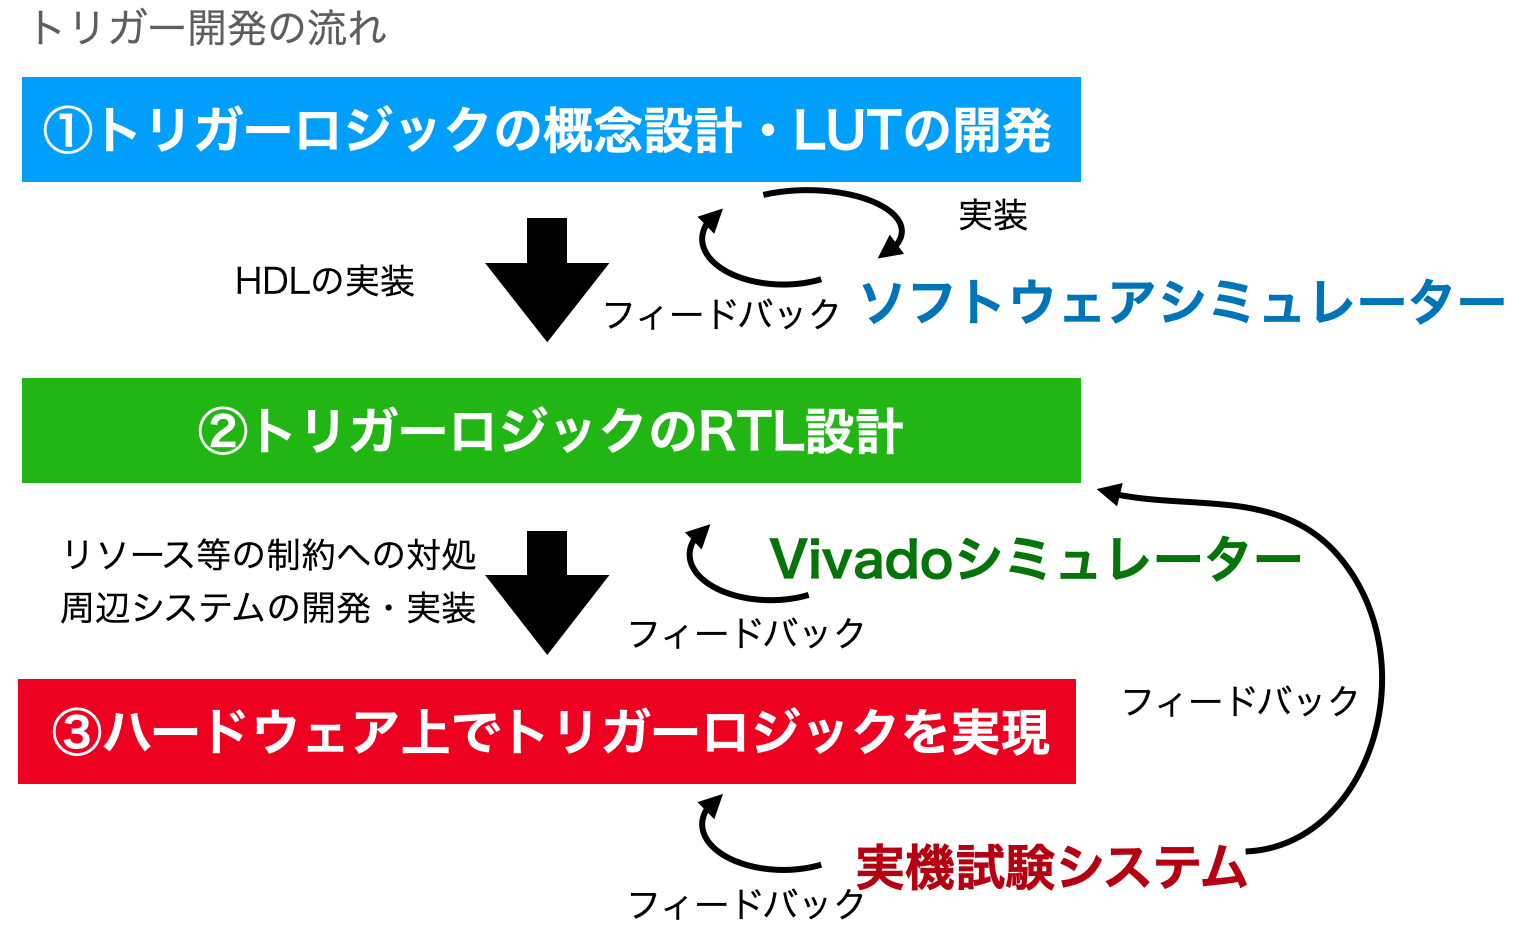
\includegraphics[width=16cm]{fig/Test/Develop_flow.png}
\caption[TGCトリガー開発の流れ]{TGCトリガー開発の流れ。}
\label{Develop_flow}
\end{figure}

\subsection*{トリガーロジックの概念設計}
設計されたロジックの概念を、より具体的なデザインに落とし込み、その性能を評価する作業にはソフトウェアシミュレーターが用いられた。ソフトウェアは開発が容易で、ロジックの実装→性能評価→ロジックの修正→…という開発サイクルを比較的早く回すことができる。そのため、グローバルなデザインを決めていく初期の開発では重宝された。例えば、TGC BW 7層のヒット情報をStatino Coincidenceにより3つの代表点に絞り、その後パターンマッチングで角度情報を取得する、などの大枠の設計はここで決められた。また、各コインシデンスロジックの最小単位であるユニットの定義や、Segment Reconstructionで複数の飛跡候補が存在する時に、ヒットレイヤーの多さを基準に候補を絞る、などの具体的なデザインもここで決められた。さらに、パターンマッチングに利用されるLUTもロジックの設計と同時にソフトウェア的に開発されており、ソフトウェアシミュレーターはLUTも含めたトリガーロジックの性能評価を行っている。

図\ref{Soft_WS}にソフトウェアシミュレーターで測定された、TGC BW コインシデンスのトリガー効率を示す。トリガー効率の評価にはSingle Muon MCサンプルが用いられた。このイベントにはフォワードおよびエンドキャップ領域 ($1.05 < | \eta | < 2.4$) 、$\phi$全領域 (-3.14 < $\phi$ < 3.14) が含まれる。MCサンプルに含まれるTGC チェンバーのヒットチャンネル情報をトリガーロジックのインプットとして利用している。Efficiencyは以下のように定義され\pt 閾値ごとにビンわけされている。

\begin{equation}
\mathrm{Efficiency} = \frac{\mathrm{TGC\,BW\,coincidenceで}\,p_{\mathrm{T}}\,閾値20、15、10、5\,\mathrm{GeV}と判断されたミューオンの数}{オフラインで再構成されたミューオンの数}
\end{equation}

プラトー領域でのEfficiencyは94 \%程度で、高い検出効率を貯まっている。また閾値より低い\pt のミューオンを効率的に削減することができている。

\begin{figure} 
\centering
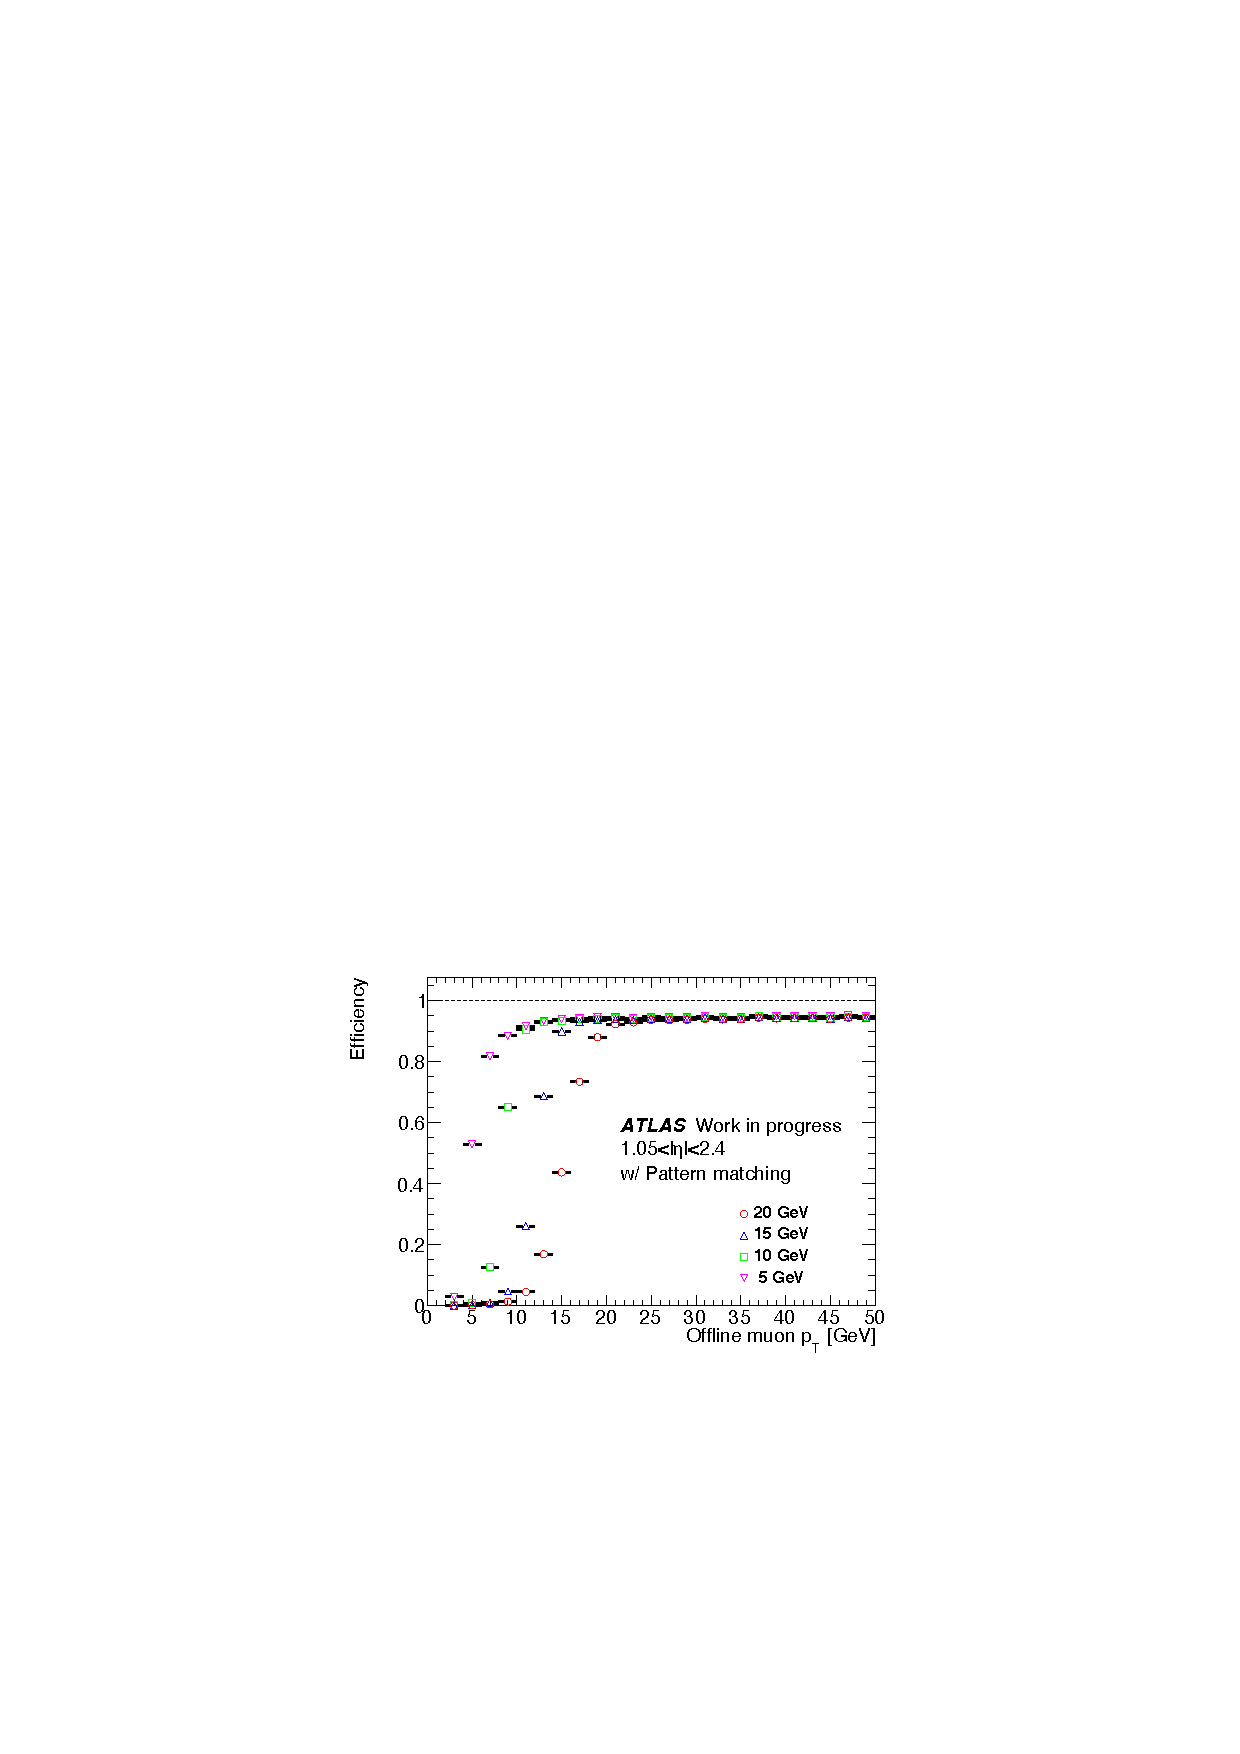
\includegraphics[width=16cm]{fig/Test/Soft_WS.pdf}
\caption[ソフトウェアシミュレーターで測定された、Wire Strip Coincidenceのトリガー効率]{ソフトウェアシミュレーターで測定された、Wire Strip Coincidenceのトリガー効率\cite{SLPDR}}
\label{Soft_WS}
\end{figure}

\subsection*{トリガーロジックのRTL実装}
次に開発されたロジックを実現するRegister Transfer Level (RTL) の設計が進められた。この過程ではソフトウェアで記述された論理を、Hardware Description Language (HDL) と呼ばれるデジタル回路における信号遷移におとしこむ作業が行われた。開発されたRTLの動作検証および実装されたトリガー回路の性能評価には、Vivado シミュレーターが用いられる。Vivado シミュレーターとはHDLで記述されるデジタル回路の動作をエミュレートするソフトウェアツールで、ロジック全体の信号の遷移を厳密にシミュレーションし、任意の信号をプローブすることができる。

Vivado シミュレーターで行われた各モジュールの性能評価の結果を述べる。Wire Segment Reconstructionの性能評価の結果を図\ref{Vivado_Wire_Efficiency}に示す。この試験でも同様のSingle Muon MCサンプルが利用され、イベント数は150,000 である。MCサンプルに含まれるTGC チェンバーのヒットチャンネル情報をWire Station Coincidenceのインプットに適したフォーマットに整形し、それに対する応答を調査しているEfficiencyは以下のように定義され、Truth Muonの$\eta$、$\phi$ごとにビンわけされている。

\begin{figure}
\begin{minipage}[b]{.5\linewidth}
\centering
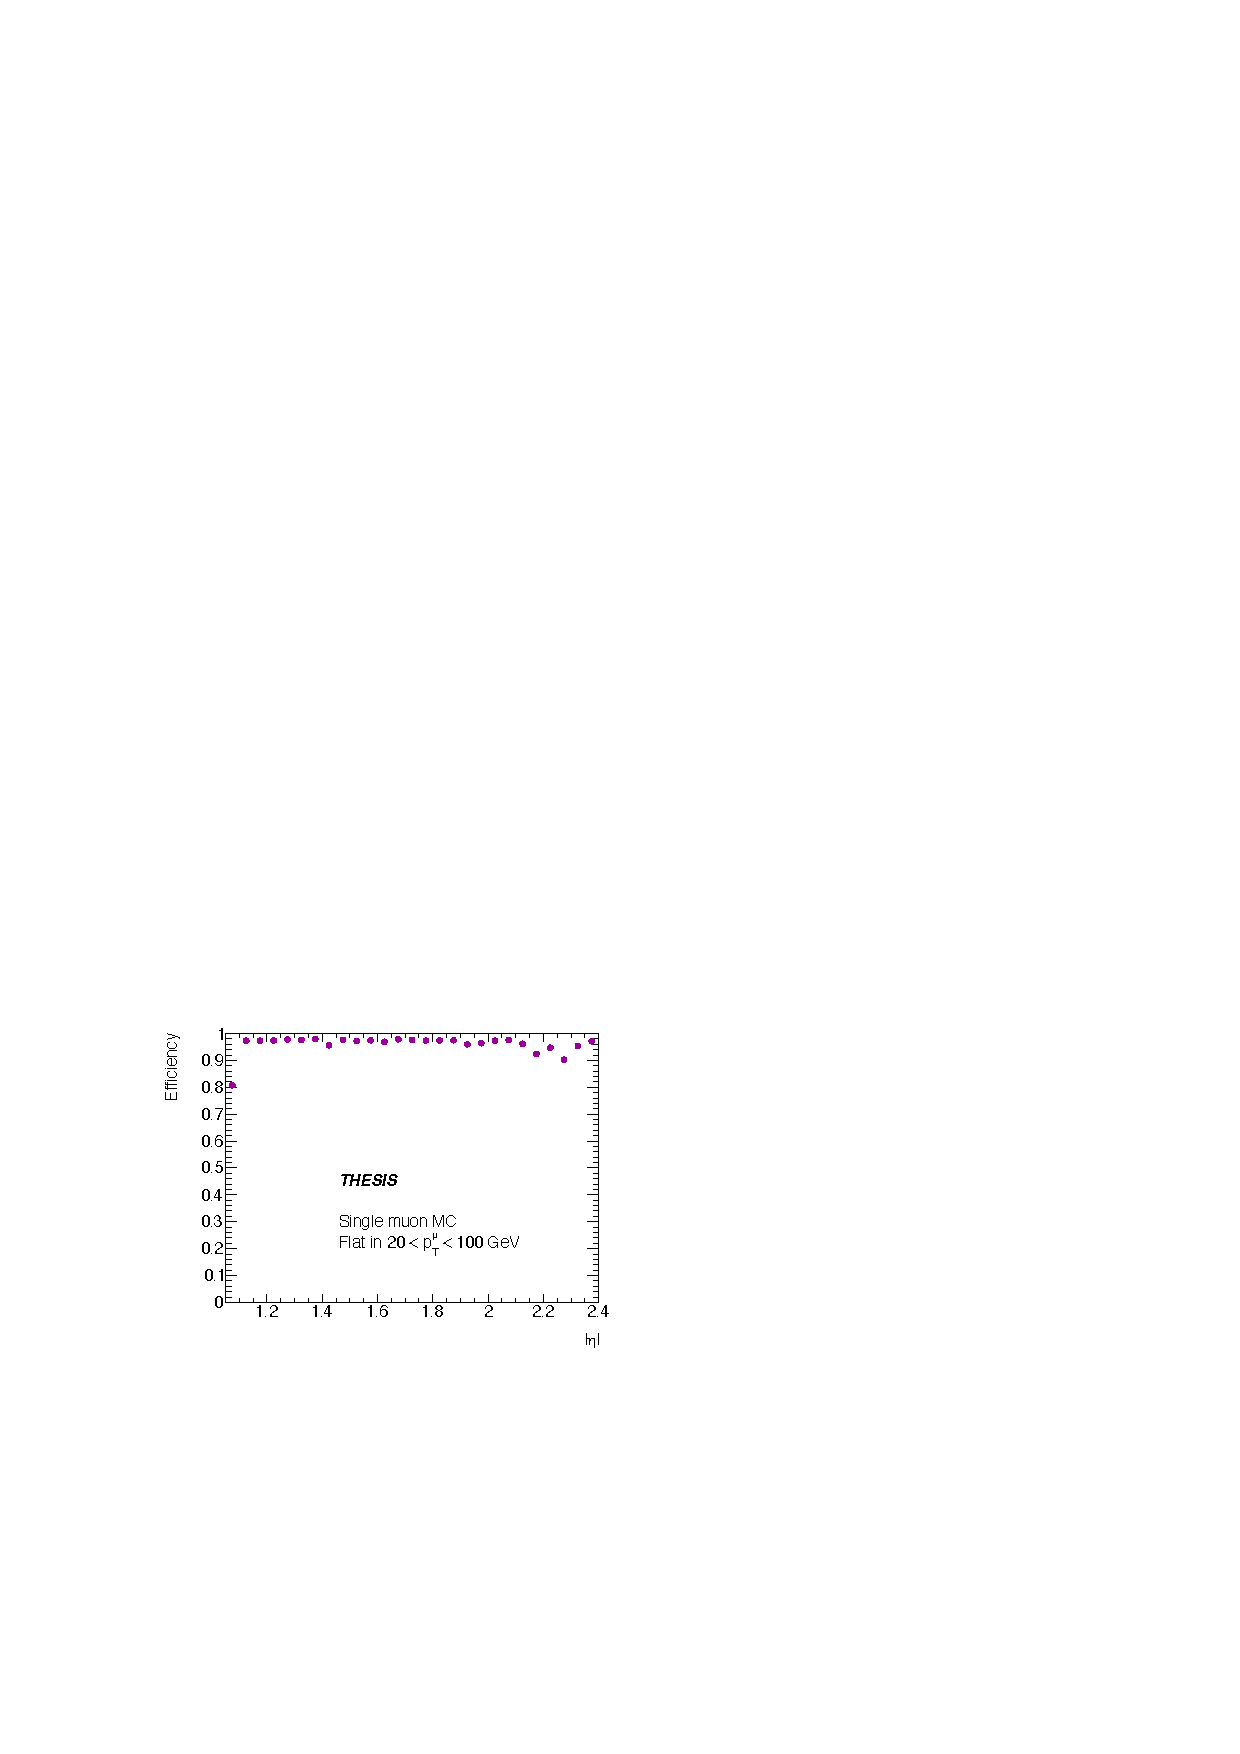
\includegraphics[height=6cm]{fig/Test/Vivado_Wire_eta.pdf}
\subcaption{Efficiencyの$\eta$依存性}
\end{minipage}%
\begin{minipage}[b]{.5\linewidth}
\centering
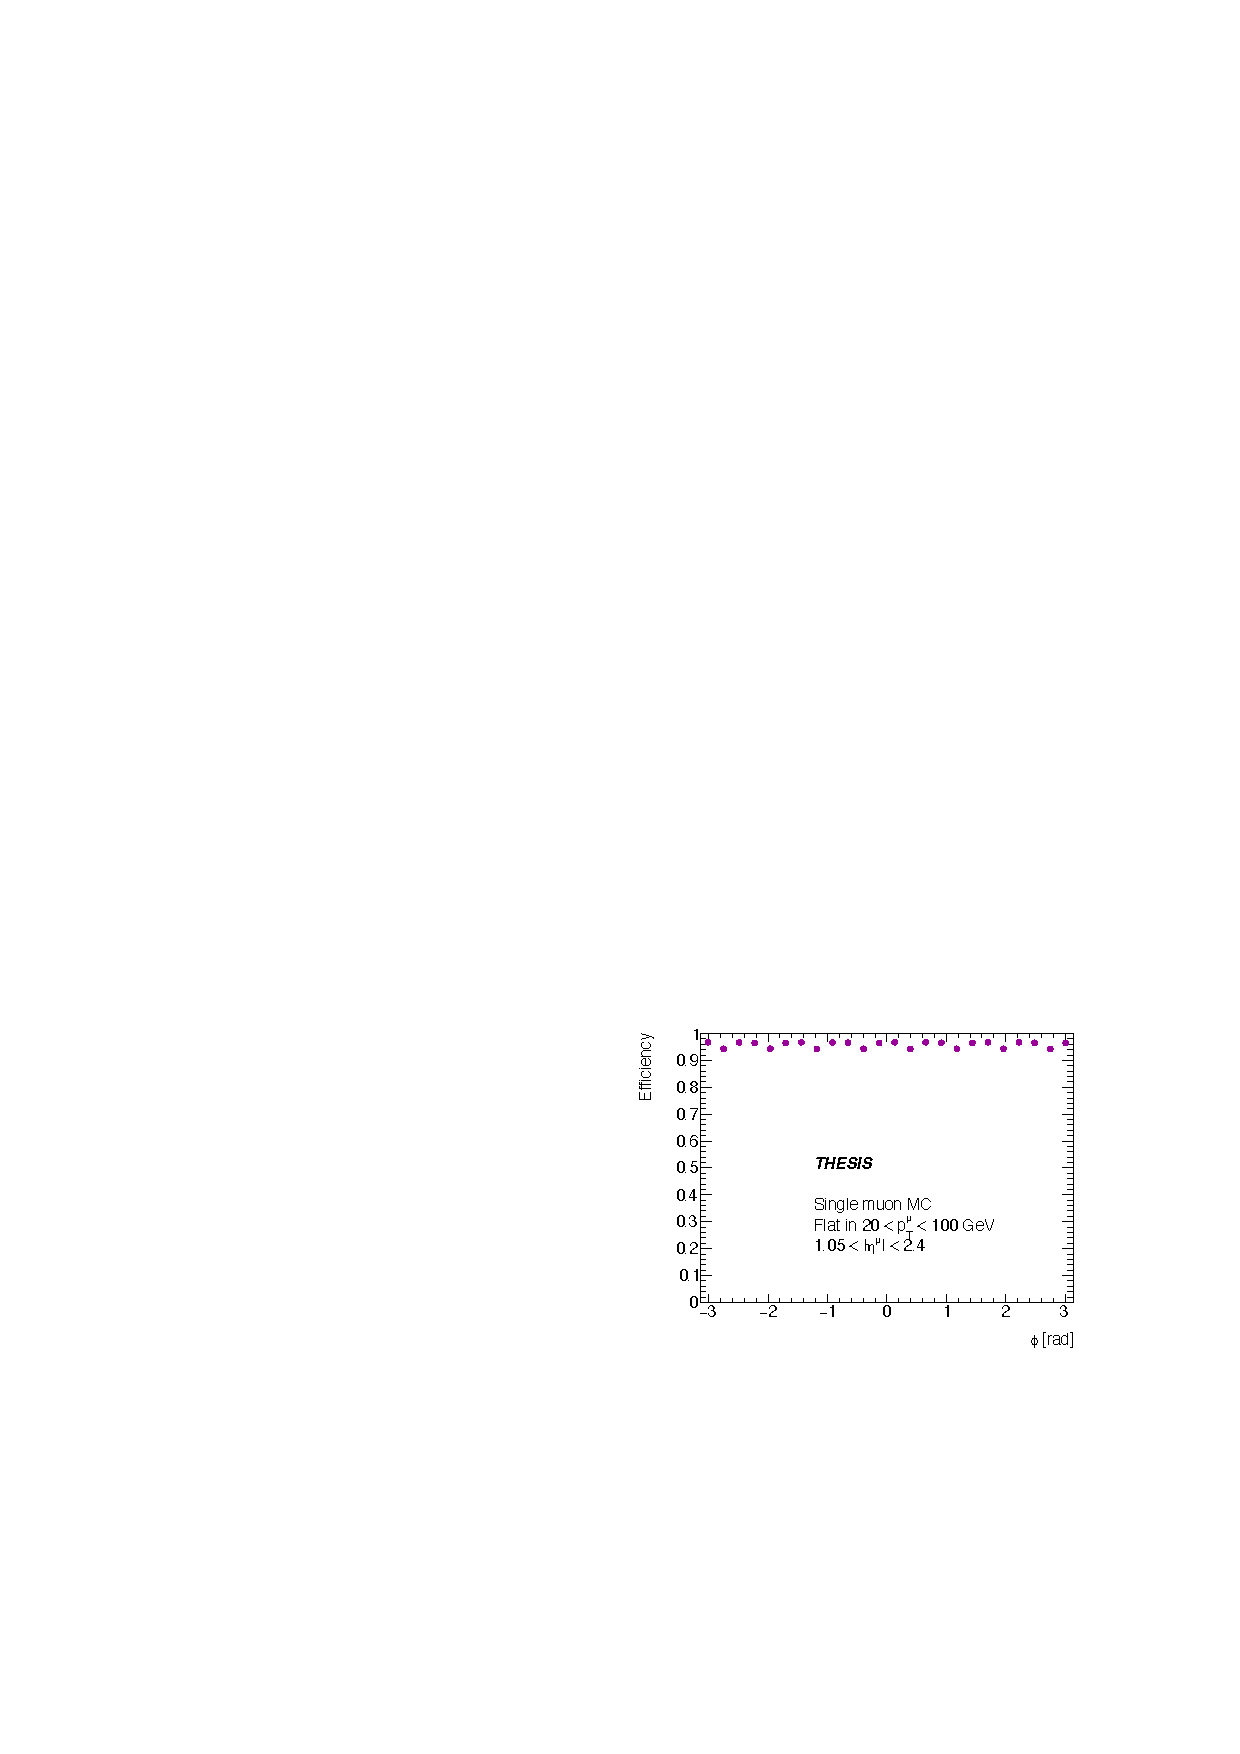
\includegraphics[height=6cm]{fig/Test/Vivado_Wire_phi.pdf}
\subcaption{Efficiencyの$\phi$依存性}
\end{minipage}%
\caption[Wire Segment Reconstructionの検出効率]{Wire Segment Reconstructionの検出効率\cite{mt_nabeyama}}
\label{Vivado_Wire_Efficiency}
\end{figure}

\begin{equation}
\mathrm{Efficiency} = \frac{\mathrm{Wire \,Segment \,Reconstructionで}\,\Delta\theta\,\mathrm{を再構成できたイベント数}}{\mathrm{Truth ミューオン の数}}
\end{equation}


TGCチェンバーの構造やエンドキャップマグネットとの干渉によると考えられる、数\%のInefficiencyが局所的に見られるものの、Efficiencyは$\eta$、$\phi$全領域で95 \%程度に達している。これによりWIre Segment ReconstructionのHDL実装が期待通り達成されていることが検証された。

HDL実装された Strip Segment Reconstruction と Wire strip Coincidence の動作検証は、ソフトウェアシミュレーターの出力との一致を確かめることで行われた。Strip Segment Reconstruction ではソフトウェアシミュレーターによるStrip Station Coincidenceの出力をインプットとして利用し、Segment Reconstruction の出力をソフトウェアシミュレーターとVivado シミュレーターで比較している。比較結果を表\ref{tab:Vivado_strip}に示す。エンドキャップ領域 (EC) 、フォワード領域 (FW)それぞれで出力の96 \%程度は一致している。数\%の不一致は、Segment Reconstructionをパスした飛跡候補が複数あった場合にどれを優先的に後段に送るか、という候補選択ロジックの差異によるものであると理解されている。同じユニット内でヒットレイヤー数が同じ、かつユニット中心からの距離も同じである候補が存在する場合、HDLではM3 スタッガードチャンネルの上位bitを優先に選ぶ、というロジックが実装されているがソフトウェアシミュレーターではその二つを仕分ける方法を用意するのが原理的に困難である。


\begin{table}[]
    \centering
    \caption*{Strip Segment Reconstruction出力のソフトウェアシミュレーターとVivadoシミュレーター比較結果。ECはエンドキャップ領域、FWはフォワード領域を示す。\cite{mt_kawamoto}}
    \label{tab:Vivado_strip}
    \begin{tabular}{|c|cc|}
    \hline
    \multirow{2}{*}{}        & \multicolumn{2}{c|}{割合}                \\ \cline{2-3} 
                             & \multicolumn{1}{c|}{EC}      & FW      \\ \hline\hline
    飛跡情報が一致したイベント            & \multicolumn{1}{c|}{96.8 \%} & 97.8 \% \\ \hline
    候補の選び方の違いに由来する差異があったイベント & \multicolumn{1}{c|}{3.2 \%}  & 2.2 \%  \\ \hline
    候補の選び方以外に由来する差異があったイベント  & \multicolumn{1}{c|}{1.8 \%}  & 0 \%    \\ \hline
    \end{tabular}
\end{table}

Wire Strip Segment Reconstruction はソフトウェアシミュレーターのWire Segment Reconstruction、Strip Segment Reconstruction の出力を取り出してインプットとしている。比較結果を表\ref{tab:Vivado_WS}に示す。同様のわずかなロジックの違いによる出力の不一致は存在するが、おおむねソフトウェアで設計されたロジックと同等のものをHDLで実装できていることが確認された。

% Please add the following required packages to your document preamble:
% \usepackage{multirow}
\begin{table}[]
    \centering
    \caption*{Wire Strip Coincidence出力のソフトウェアシミュレーターとVivadoシミュレーター比較結果。ECはエンドキャップ領域、FWはフォワード領域を示す。\cite{mt_kawamoto}}
    \label{tab:Vivado_WS}
    \begin{tabular}{|c|cc|}
    \hline
    \multirow{2}{*}{}                      & \multicolumn{2}{c|}{割合}                \\ \cline{2-3} 
                                           & \multicolumn{1}{c|}{EC}      & FW      \\ \hline\hline
    飛跡情報が一致したイベント                          & \multicolumn{1}{c|}{98.4 \%} & 99.9 \% \\ \hline
    飛跡情報の異なったイベント                          & \multicolumn{1}{c|}{1.6 \%}  & 0.07 \% \\ \hline
    イベントで最大の\textbackslash{}pt出力がことなったイベント & \multicolumn{1}{c|}{0.09 \%} & 0.02 \% \\ \hline
    \end{tabular}
\end{table}

\subsection*{トリガーロジックのハードウェアでの実現}
最後にRTLで実装されたトリガー論理回路をハードウェア上で実現するためのインプリメンテーション作業が行われた。論理回路をハードウェア上で実現するため前章に述べたような、FPGAのリソースやタイミングの制約を満たす形での最適化が行われた。また、トリガー回路へどのように信号を入力し、演算結果をどのように取り出すかという、周辺システムの設計・実装も行われた。

しかし、実機上で動作するトリガー回路の動作検証、性能評価には工夫が必要となる。トリガー回路の入力はPS boardから受信する光信号で、出力はFelixに送信する光信号である。このままではPS boardやFelix、さらに後段の読み出し回路が完成するまで、ハードウェア上で動いているトリガー回路を検証するすべがない。

そこで本研究では、ハードウェア上で動作するトリガー回路にPS boardからの出力をエミュレートしたテストパターンを投入し、その出力をMPSoCから読み出す、シングルボード試験システムを開発した。この試験システムと、先行研究で開発されたテストパターン生成機構を用いることで、トリガー回路を限りなく本番運用に近い形で試験することができる。Vivado シミュレーター、ソフトウェアシミュレーターでこれまで行われていた試験と、本システムで達成する試験システムのフローの違いを図\ref{Test_Flow}に示す。

\begin{figure}
\begin{minipage}[b]{0.9\linewidth}
\centering
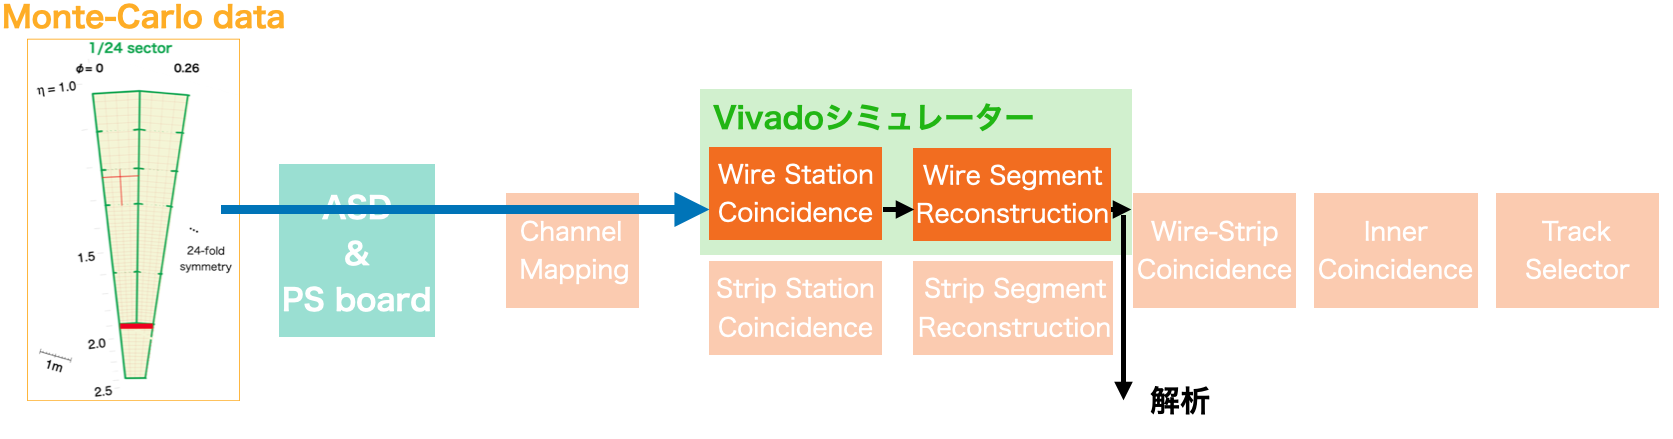
\includegraphics[height=4.8cm]{fig/Test/Flow_Wire.png}
\subcaption{Vivadoシミュレーターによる試験フロー : Wire Segment Reconstruction}
\end{minipage}\\
\begin{minipage}[b]{0.9\linewidth}
    \centering
    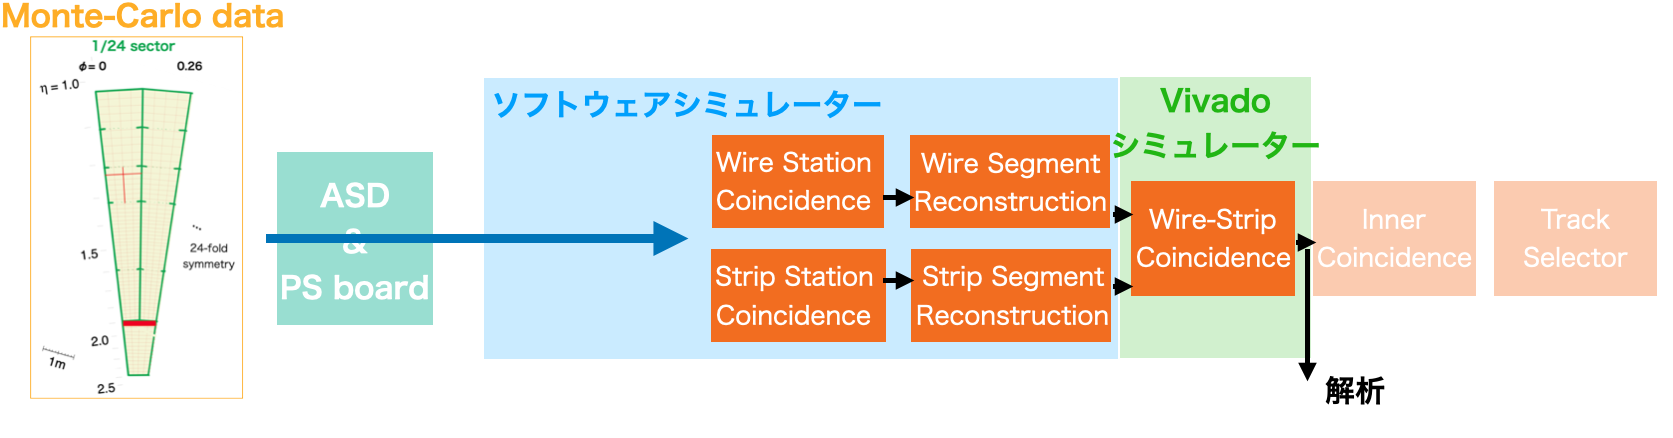
\includegraphics[height=4.8cm]{fig/Test/Flow_WS.png}
    \subcaption{Vivadoシミュレーターによる試験フロー : Wire Strip Coincidence}
\end{minipage}\\
    \begin{minipage}[b]{0.9\linewidth}
        \centering
        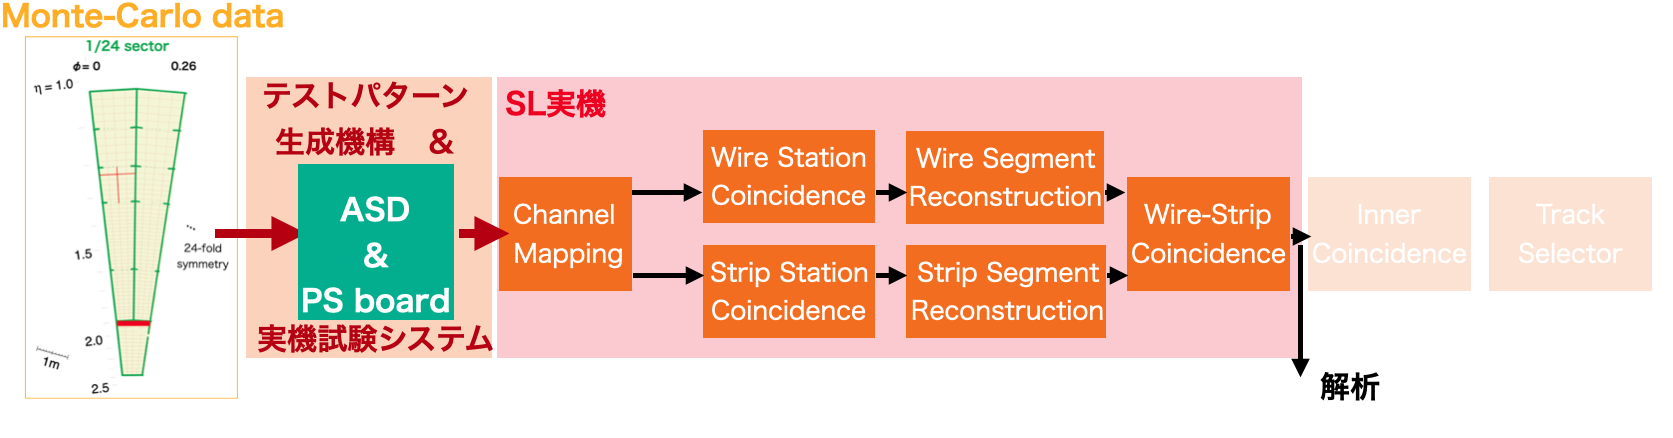
\includegraphics[height=4.8cm]{fig/Test/Flow_zikki.png}
        \subcaption{実機試験システムによる試験フロー}
    \end{minipage}\\

\caption[試験フロー]{Vivado シミュレーター、ソフトウェアシミュレーターによる試験フローと実機試験フローの比較。}
\label{Test_Flow}
\end{figure}


これまでの試験はMCサンプルやソフトウェアシミュレーターから、各モジュールのインプットを直接生成し、トリガーロジックの一部分のHDLをVivadoシミュレーターで試験していた。本試験システムではTGCのヒット情報から、フロントエンドエレクトロニクスの複雑な配線情報も考慮した上で、PS boardからSLに送られる8,000 bitのヒット情報を完全に再現し、トリガーロジックのインプットとする。それをもとにTGC BW コインシデンスをフルチェーンで動作させ、実際にハードウェア上で計算されたトリガー出力を読み出す。また、ソフトウェアシミュレーターではパターンマッチング用のLUTは最終出力のテキストファイルではなく、もととなるrootファイルを利用する。本試験ではいくつかの処理を経て、最終的に出力された本番で使われるテキストファイルを利用するためLUTの最終検査も行うことができる。

さらに、シングルボード試験を実現するには、LUTの書き込みやTTC信号の調整などのコントロールパスと、MPSoCから読み出すための読み出しパスも、トリガー回路と同期しながら精度よく動作する必要があり、SL FPGAの総合的な動作検証を行うことができる。

加えて、実機試験システムはトリガー演算をFPGA上で行っているため、Vivado シミュレーターと比べて高速で動作する。これにより、大統計を活かした網羅的な検証も可能で、これまでVivado シミュレーターでは発見することができなかった局所的な不具合の発見も期待される。\footnote{Vivado シミュレーターはデジタル回路の全ての信号遷移をソフトウェア的に計算するため、回路規模が大きくなると動作が遅くなる。ファームウェア全体をシミュレーションすると、数10イベントに半日程度かかることがわかっており、高統計の試験はできなかった。}

次節で開発した実機試験システムおよびテストパターン生成機構の詳細を説明する。

\section{実機試験システム}

\subsection*{実機試験システムの概要}
\label{subsec_TestSystemOverview}
図\ref{Test_system}に実機を用いた試験システムの全体像を示す。このシステムは主にテストパターン生成システム、実機試験システム、Bit-wiseシミュレーターで構成される。実機試験システムは本研究で開発を進めた。テストパターン生成システムおよびBitwiseシミュレーターは先行研究で開発された。以下にそれぞれの詳細を説明する。

\begin{figure} 
\centering
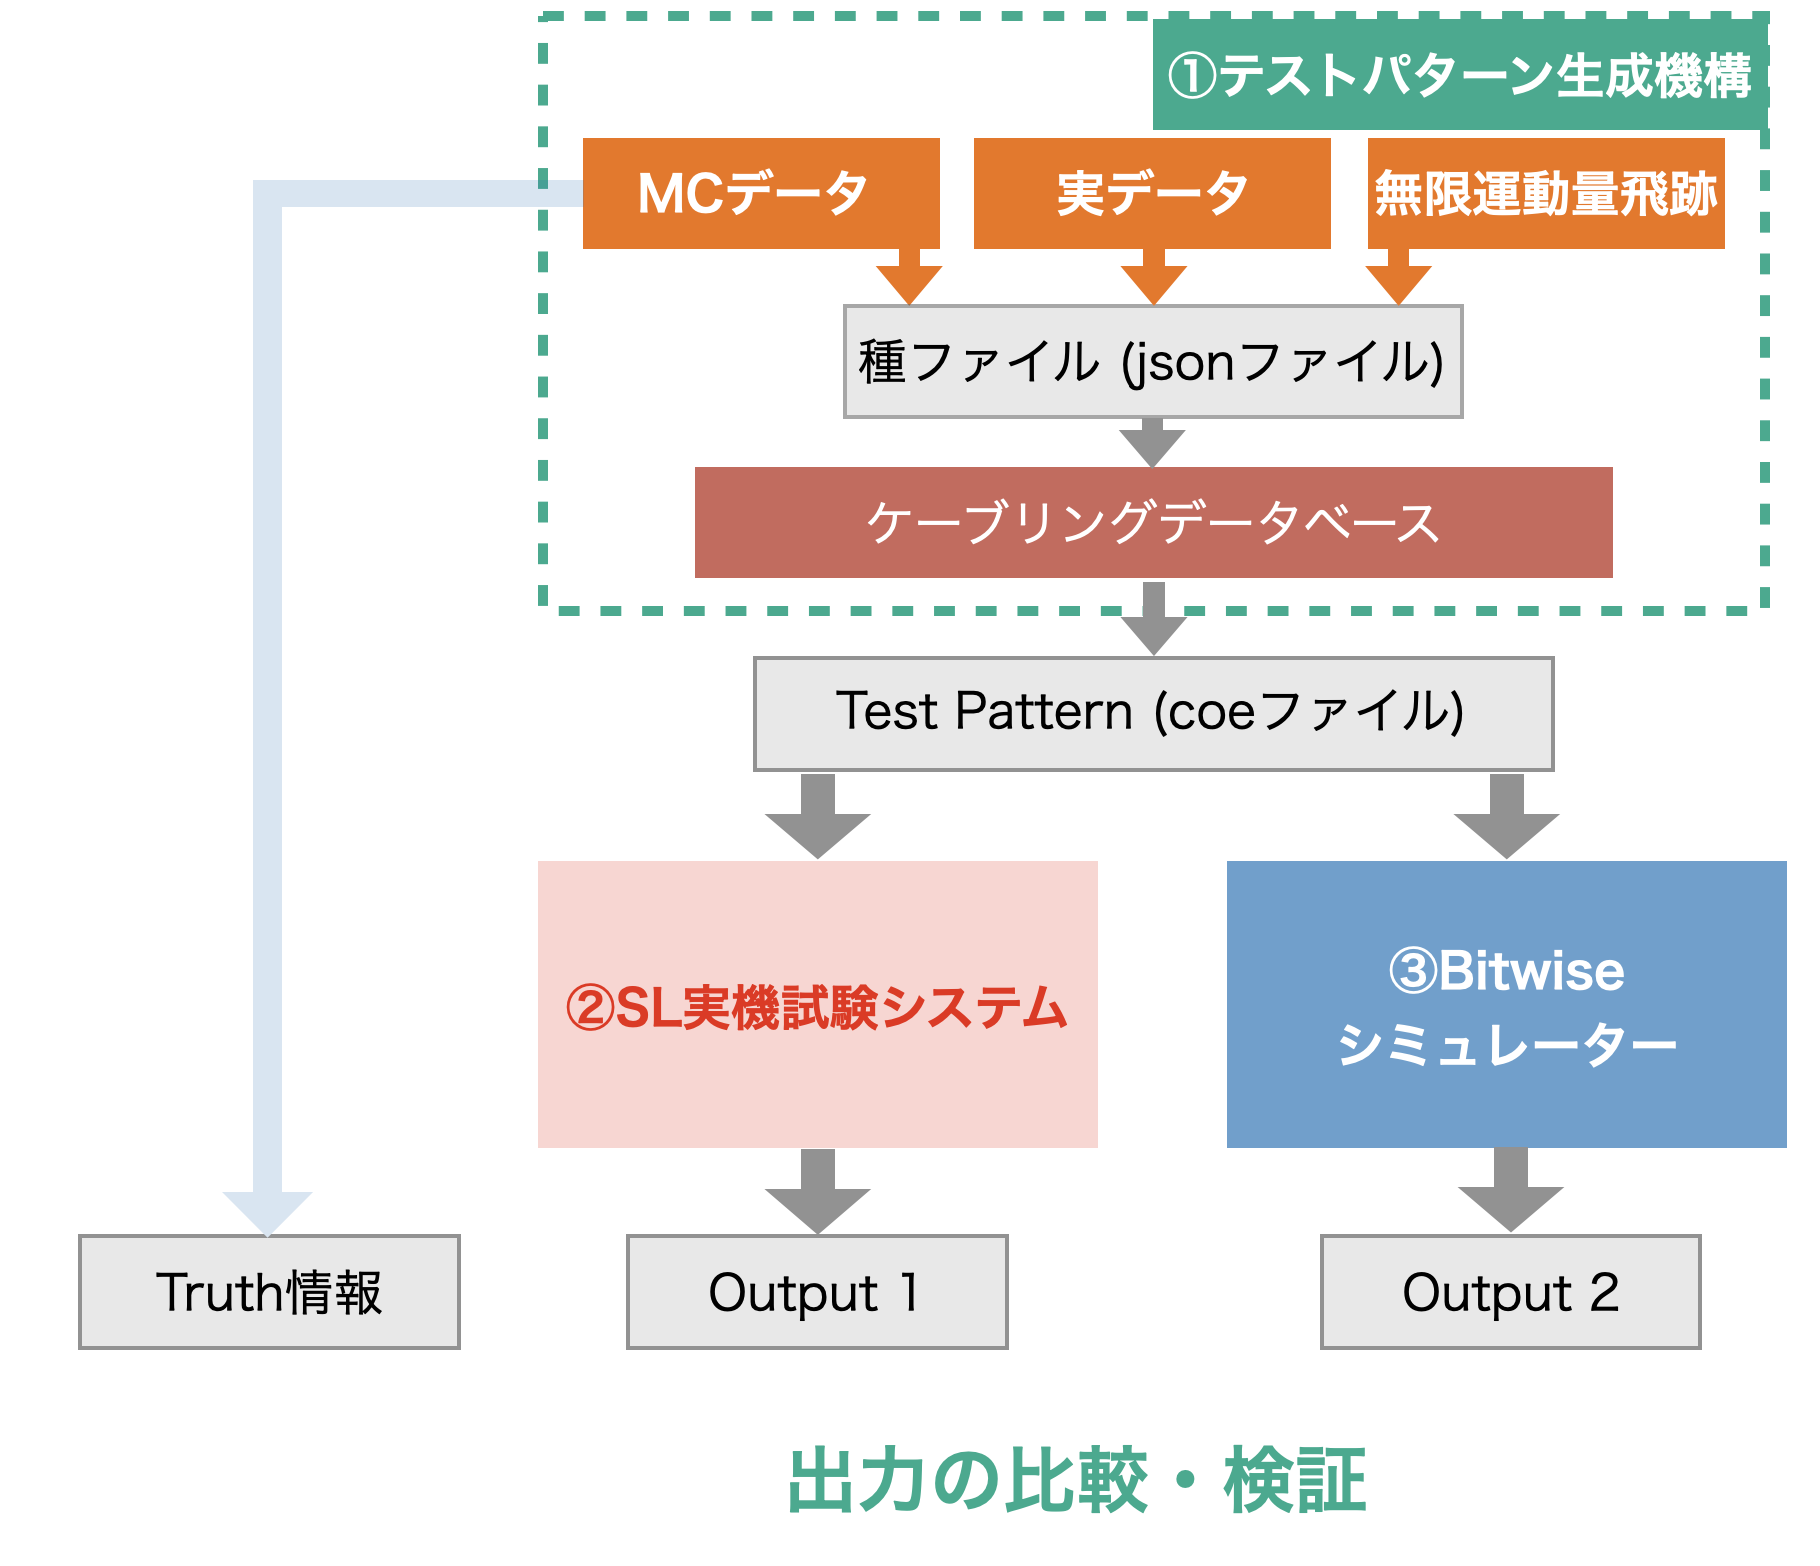
\includegraphics[width=16cm]{fig/Test/Test_system.png}
\caption[実機試験システムの概要]{実機試験システムの概要}
\label{Test_system}
\end{figure}

\paragraph{テストパターン生成システム}  
\par
\ref{}節で述べたようにSLは、1枚のPS boardから2本の光ファイバーを通じて128 bit x 2 ファイバーのヒット信号を受け取る。1枚のSLは合計 29枚のPS boardと接続するため、イベントごとに128 bit x 58 ファイバーのヒットビットマップがトリガーロジックに入力される。モンテカルロシミュレーションや過去のRunで取得された、TGCのヒットチャンネルの情報から、トリガーロジックに入力されるヒットビットマップをエミュレートする仕掛けが、テストパターン生成システムである。

テストパターン生成システムは、元のデータセットに格納されている、各イベントにおけるTGC検出器のチャンネルごとのヒット情報を抽出し、テストパターンの種ファイルとしてjsonファイルに格納する。この際、モンテカルロデータ、実データ、toyデータなどいかなるデータセットも統一的なフォーマットでjsonファイルを作成することで、この後の処理はその違いに関わらず進めることができる。生成されたjsonファイルはケーブリングデータベースと接続される。ケーブリングデータベースはTGC検出器からSLまでの複雑な配線情報 (ASD、PS board、SLと続く物理的なケーブルの配線に加え、各デジタル回路内の信号の並び替え情報等も含む) を一元的に管理しているデータベースである。この2つを合わせることで、任意のデータセットからSLのインプットを再現したテストパターンを生成することができる。テストパターンはSL実機、Vivado シミュレーション、後述するBitwiseシミュレーターに共通して入力できるようにcoeファイル形式で出力される。これにより、全く同じインプットを3つのシミュレーターに食わせる、コヒーレントな検証が可能になっている。

\paragraph{実機試験システム}  
\par
実機試験システムは生成されたテストパターンをインプットに、実際にハードウェア上でトリガー回路を動作させ、その出力を取り出すシングルボード試験システムである。その詳細は次節説明する。

\paragraph{Bitwiseシミュレーター}  
\par
BitwiseシミュレーターはSLトリガーロジックをビットレベルで再現したC++ベースのシミュレーターである。このシミュレーターはテストパターンを入力とし、LUTもテキストファイルとしてダンプされた最終生成物を使用するため、実機システムと完全に等価な試験を実現することができる。そのため、実機システムとの比較・検証用に極めて有用である。また、各モジュールのロジックや入出力もファームウェアと完全に一致するように設計されているため、途中出力同士の比較や、実機出力では出せない内部の信号線の調査にも利用することができ、HDLの精密なデバッグが可能である。\footnote{前述のソフトウェアシミュレーターは実現しているロジックはファームウェアと完全に等価であるが、入力データやLUTは実機システムとは異なるため、最終的な動作確認には不向きである。また内部でビットレベルの演算を行なっている訳ではないので、途中出力をファームウェアと比較することもできない。}

\subsection{実機試験システムの開発}
\subsubsection*{ファームウェアの概要}
図\ref{}に実装したトリガーロジック試験システムの概要を示す。試験システムのコントロールおよびデータ読み出しはMPSoC上のLinuxを起点に行う。本システムではSL単体での試験を実現するため、SL上の水晶発振器で生成した40.079 MHzクロックをLHC陽子バンチ交差クロックの代わりに基準クロックとして扱う。FELIXから配られるTest Pulse Trigger (TPT)やL0AなどのTTC信号もSL内部のTTC emulatorで擬似的に生成し、各モジュールに分配する。

PS boardから受信するヒット信号をエミュレートしたテストパターンは、Test Pattern Generator内のBRAMに格納される。Test Pattern GeneratorはTTC emulatorからTest Pulse Trigger (TPT) 信号を受信すると、1イベント分のヒットビットマップをトリガー回路に投入する。Trigger Logicからの出力はLHCバンチ交差クロックに同期してL0 Bufferにダンプされ、読み出し回路を経てMPSoC上のLinuxから読み出される。トリガー回路のは固定レイテンシーで動作するため、TTC emulatorはTPTから決まったクロックチック後にL0Aを出すことで、TPTに該当するトリガ出力を読み出すことができる。以下に各モジュールの概要を説明する。

\paragraph{Test Pattern Generator}  
\par
Test Pattern Generator は幅 128 bit、深さ 64 のBRAMで、1つのBRAMがPS board 1リンク分の信号をエミュレートする。全31 PS board x 2リンクの信号をエミュレートするために合計62個のBRAMが並列に配置されている。トリガーロジックや読み出し回路にTest patternを入力するか、PS baordから受信したデータを入れるかはスイッチで切り替えられるようになっている。テストパターンはcoe形式のファイルを用いてBRAMの初期値として設定できることに加え、\ref{}節で述べたLUT書き込み機構と同様の仕組みにより、コントロールパスからも書き換え可能である。これによりBRAMの深さ64に制限されることなく、任意のイベント数での試験が可能になっている。

\paragraph{トリガーロジック}  
\par
トリガー回路の出力は読み出し用のフォーマットに整形され、トリガー読み出し回路へ渡される。今回の試験では各モジュールの動作を詳細に調査するため、モジュール間で受け渡される全てのビットマップを読み出せるようフォーマットを定義している。例としてWire Strip Coincidenceの読み出しデータを説明する。Wire Strip Coincidenceは44の8 regionと34の32 regionで構成され、160 MHzクロックに同期して、8regionから最大1つ、32 regionから最大4つのミューオン候補がInner Coincidenceに送られる。読み出し回路でもこの最大180のミューオン候補を並列に読み出せるよう設計しており、各領域ごとに表\ref{tab:WS_format}の形式にフォーマットしたデータを読み出し回路に送信する。各モジュールの出力フォーマットでは最上位1bitはvalid信号を定義するようにする。後述の読み出し回路ではこのvalid信号が立てられているユニットの出力だけを読み出す設計にしている。

\begin{table}[]
    \centering
    \caption[Wire Strip Coincidenceの読み出しフォーマット]{Wire Strip Coincidenceの読み出しフォーマット。}
    \label{tab:WS_format}
    \begin{tabular}{|c|c|}
    \hline
    \# of bits & Name                                            \\ \hline\hline
    1          & Valid flag                                      \\ \hline
    4          & $p_{\mathrm{T}}$                                \\ \hline
    3          & 0                                               \\ \hline
    7          & $\Delta\theta$ from Wire Segment Reconstruction \\ \hline
    2          & Wire Matched Layer                              \\ \hline
    4          & $\Delta\phi$ from Strip Segment Reconstruction \\ \hline
    2          & Strip Matched Layer                             \\ \hline
    1          & 0                                               \\ \hline
    \end{tabular}
\end{table}


それぞれのトリガーモジュールから読み出すデータの出力ビット幅を表\ref{tab:output_width}に示す。ビット幅の大きな出力を後段の読み出しロジックに一斉にダンプすると、タイミング制約を満たすことが難しくなるため、そのような出力はいくつかの並列なレーンに分割して処理している。

\begin{table}[]
    \centering
    \caption[各モジュールの出力ビット幅]{各モジュールの出力ビット幅。}
    \label{tab:output_width}    
    \begin{tabular}{|c|c|c|c|}
    \hline
    トリガーロジック                                      & SLR & 出力ビット幅 (bits) & レーン数 \\ \hline\hline
    \multirow{3}{*}{Channel Mappin}               & 0   & 2732          & 4    \\ \cline{2-4} 
                                                  & 2   & 2732          & 4    \\ \cline{2-4} 
                                                  & 3   & 1000          & 2    \\ \hline
    \multirow{3}{*}{Wire Station Coincidence}     & 0   & 1768          & 3    \\ \cline{2-4} 
                                                  & 2   & 1768          & 3    \\ \cline{2-4} 
                                                  & 3   & 804           & 3    \\ \hline
    \multirow{3}{*}{Strip Station Coincidence}    & 0   & 1890          & 3    \\ \cline{2-4} 
                                                  & 2   & 1890          & 3    \\ \cline{2-4} 
                                                  & 3   & 378           & 3    \\ \hline
    \multirow{3}{*}{Wire Segment Reconstruction}  & 0   & 3404          & 5    \\ \cline{2-4} 
                                                  & 2   & 3404          & 5    \\ \cline{2-4} 
                                                  & 3   & 1472          & 2    \\ \hline
    \multirow{3}{*}{Strip Segment Reconstruction} & 0   & 360           & 1    \\ \cline{2-4} 
                                                  & 2   & 360           & 1    \\ \cline{2-4} 
                                                  & 3   & 72            & 1    \\ \hline
    \multirow{3}{*}{Wire Strip Coincidence}       & 0   & 1776          & 3    \\ \cline{2-4} 
                                                  & 2   & 1776          & 3    \\ \cline{2-4} 
                                                  & 3   & 768           & 1    \\ \hline
    \end{tabular}
\end{table}

全てのトリガーロジックの読み出し回路を同時に実装するのはリソースの観点で不可能である。読み出したいデータをリンクごとに選択し、目的に応じて異なるファームウェアを用意して試験を行う。例えばFW領域のロジックを重点的に調べたい場合には、SLR3のStation CoincidenceからWire Strip Coincidenceまでのリンクを選択する。一方、SLR0、SLR2、SLR3それぞれでWire Segment Reconstructionを出力させることも可能である。実験本番で用いるファームウェアでは、各トリガーロジックからの出力から必要最低限の情報を抜き出すことで、全てのトリガーロジックの読み出し回路を同時に実現する予定である。

\paragraph{トリガー読み出し回路}  
\par
\begin{itemize}
    \item L0 Buffer 
    トリガーロジックでフォーマットされたデータはL0 Bufferにダンプされる。L0 Bufferは入力ビットマップと同じ幅をもつ深さ512のBRAMでであり、TTC emulatorからL0Aが出されるまでのバッファリングを行う。トリガーロジックには40 MHz、160 MHz、240 MHzで駆動するものが存在する。いずれの場合でも1つの陽子バンチ衝突由来の出力は25 nsごとに横並びに揃えられ、40 MHzのLHC クロックで動作する書き込みポインタに従って、L0 Bufferに格納される。一方、読み出しは240 MHzで行われ、読み出されたデータはDerandomizerに送られる。

    \item Derandomizer
    \item 
\end{itemize}

\section{無限運動量飛跡を用いた試験}
\label{sec_IMT}

\subsection{無限運動量飛跡の生成}
\label{subsec_IMT_generation}

\subsection{試験結果・問題点の整理}
\label{subsec_IMT_result}

\subsection{問題点の解決結果}
\label{subsec_IMT_solution}

\section{Single Muon Monte-Carloデータを用いた網羅試験}
\label{sec_SingleMuon}

\subsection{Single Muon Monte-Carloデータの生成}
\label{subsec_SingleMuon_generation}

\subsection{試験結果・問題点の整理}
\label{subsec_SingleMuon_result}

\subsection{問題点の解決結果}


